\subsection{UC21 - Visualizzazione errore inserimento misura}
\begin{figure}[H]
  \centering
  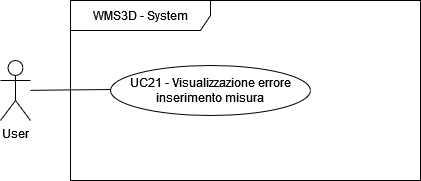
\includegraphics[width=0.8\textwidth]{UC_diagrams_21-27/UC21.drawio.png}
   \caption{Diagramma UML UC21 - Visualizzazione errore inserimento misura}
\end{figure}
\begin{itemize}
    \item \textbf{Attori:} User.
    \item \textbf{Pre-condizione:}  L'utente ha inserito in un dato di tipo misura un valore non compreso tra i valori numerici positivi razionali.
    \item \textbf{Post-condizione:} L'utente visualizza un messaggio d'errore e l'operazione fallisce.
    \item \textbf{Scenario Principale:}  L'utente visualizza un messaggio informativo sull'errore e ne conferma la ricezione. L'operazione, di conseguenza, fallisce.
    \item \textbf{Generalizzazioni:} -
    \item \textbf{Estensioni:} -
\end{itemize}